\themaN
\graphicspath{{../../S20_Somme_et_difference_de_nombres_relatifs/Images/}}

% pour créer la pyramide (#1 est le nombre de cases en bas)
\newcommand{\pyramidedenombres}[1]{
   \pgfmathparse{#1-1};
   \edef\yy{\pgfmathresult};
   \foreach \y in {0,1,...,\yy}{
      \pgfmathparse{\yy-\y};
      \edef\xx{\pgfmathresult};
      \foreach \x in {0,...,\xx}{
         \draw (\x+0.5*\y,1+\y) rectangle (\x+1+0.5*\y,0+\y);}};}

% pour placer dans la pyramide a l'étage #1 dans la case #2 le nombre #3 
\newcommand{\pyramideplacernombre}[3]{
   \pgfmathparse{0.5*#1+#2-1};
   \edef\xx{\pgfmathresult};
   \pgfmathparse{#1-0.5};
   \edef\yy{\pgfmathresult};
   \draw (\xx,\yy) node {$#3$};}

\newcommand\encercle[1]{%entourer les nombres
   \unitlength1em
   \begin{picture}(2,2)
      \put(0.75,0.3){\circle{3}}
      \put(0,0){\parbox[b]{1.5em}{\centering#1}}
   \end{picture}}
   
\chapter{Somme et différence de nombres relatifs}
\label{S20}


%%%%%%%%%%%%%%%%%%%%%%%%%%%%%%%%%%%%%%%%%
%%%%%%%%%%%%%%%%%%%%%%%%%%%%%%%%%%%%%%%%%
\begin{prerequis}
   \begin{itemize}
      \item Somme et différence de nombres décimaux.
      \item[\com] Calculer avec des nombres décimaux relatifs.
   \end{itemize}
\end{prerequis}

\vfill

\begin{debat}[Débat : Brahmagupta et l'invention du 0]
   {\bf Brahmagupta} est un mathématicien indien né en 598. Dans l'un de ses ouvrages, le {\it Brahma Sphuta Siddhanta}, il présente les règles d'arithmétique qui concernant les nombres positifs (qu'il appelle les biens) et les nombres négatifs (qu'il appelle les dettes) par des calculs de pertes et de profits. Il définit ainsi le zéro comme la différence d’un nombre par lui-même. Par exemple, voilà comment il exprime les opérations usuelles :
   \begin{itemize}
      \item zéro soustrait d’une dette est une dette ;
      \item zéro soustrait d’un bien est un bien ;
      \item zéro soustrait de zéro est zéro ;
      \item une dette soustraite de zéro est un bien ;
      \item un bien soustrait de zéro est une dette.
   \end{itemize}
   \begin{center}
      \textcolor{B1}{
      \begin{pspicture}(0,1)(11,5.5)
         \psset{fillstyle=solid}
         \psellipse[fillcolor=A1!50](2,4.3)(1.3,0.8)
         \rput(2,4.6){\it indien}
         \rput(2,4){\bf sunya}
         \psline{->}(3.5,4.3)(4.5,4.3)
         \psellipse[fillcolor=A1!40](6,4.3)(1.3,0.8)
         \rput(6,4.6){\it arabe}
         \rput(6,4){\bf sifr}
         \psline{->}(7.5,4.3)(9,3.9) %
         \psellipse[fillcolor=A1!30](9.5,3)(1.3,0.8)
         \rput(9.5,3.3){\it latin}
         \rput(9.5,2.7){\bf zephirum}
         \psline{->}(9,2.1)(7.5,1.7)
         \psellipse[fillcolor=A1!20](6,1.7)(1.3,0.8)
         \rput(6,2){\it italien}
         \rput(6,1.4){\bf zephiro}
         \psellipse[fillcolor=A1!10](2,1.7)(1.3,0.8)
         \rput(2,2){\it français}
         \rput(2,1.4){\bf zéro}
         \psline{<-}(3.5,1.7)(4.5,1.7)    
      \end{pspicture}}
   \end{center}
   \bigskip
   \begin{cadre}[B2][F4]
      \begin{center}
         Vidéo : \href{https://leblob.fr/fondamental/les-nombres-negatifs}{\bf Les nombres négatifs}, site Internet {\it Le blob}, épisode de la série {\it Petits contes mathématiques}.
      \end{center}
   \end{cadre}
\end{debat}

\vfill

\textcolor{PartieGeometrie}{\sffamily\bfseries Cahier de compétences} : chapitre 3, exercices 24 à 47.


%%%%%%%%%%%%%%%%%%%%%%%%%%%%%%%%%%%%
%%%%%%%%%%%%%%%%%%%%%%%%%%%%%%%%%%%%
\activites

\begin{activite}[La pêche mystérieuse]
   {\bf Objectif :} effectuer des additions et des soustractions avec des nombres entiers relatifs.
   \begin{QCM}
      Sept amis jouent à la fête foraine au jeu de la pêche mystérieuse, ils gagnent ou il perdent des points selon les objets qu'ils \og pêchent \fg. Voilà les points qu'ils peuvent gagner : \\
      \begin{pspicture}(0,1)(15,3.25)
         \rput(2,2.25){\psscalebox{0.4}{\psBill}}
         \rput(4,2.5){\it\textcolor{B1}{Billy}}
         \rput(4,2){\it\textcolor{B1}{+150 points}}
         \rput{-30}(6,2.4){\psscalebox{0.55}{\psBird}}
         \rput(9.5,2.5){\it\textcolor{B1}{Birdy}}
         \rput(9.5,2){\it\textcolor{B1}{+100 points}}
         \rput(12.5,1.5){\psKangaroo[fillcolor=brown]{1.7}}
         \rput(14.5,2.5){\it\textcolor{B1}{Skippy}}
         \rput(14.5,2){\it\textcolor{B1}{+50 points}}
      \end{pspicture} \\
      Cependant, certains objets font perdre des points : \\
      \begin{pspicture}(0,1)(15,3.25)
         \rput{-30}(2.2,2.25){\psscalebox{0.4}{\psAnt}}
         \rput(4,2.5){\it\textcolor{B1}{Antas}}
         \rput(4,2){\it\textcolor{B1}{-25 points}}
         \rput(6.7,1.7){\psscalebox{0.25}{\psFish[fillstyle=slope]}}         
         \rput(9.5,2.5){\it\textcolor{B1}{Fishas}}
         \rput(9.5,2){\it\textcolor{B1}{-75 points}}
         \rput(12.6,2.5){\psscalebox{0.45}{\psPig[fillcolor=pink](0,0)}}
         \rput(14.5,2.5){\it\textcolor{B1}{Pigas}}
         \rput(14.5,2){\it\textcolor{B1}{-125 points}}
      \end{pspicture} \\
      Compléter le tableau suivant des gains et des pertes. En déduire le total, puis le classement.
      \begin{center}
         \begin{Ltableau}{0.9\linewidth}{4}{c}
            \hline
            Pêche & Gains & Pertes & Total \\
            \hline
            \begin{pspicture}(0,1.5)(9.5,3)
               \rput[l](0,2.2){Smaïl}
               \rput(2,2.25){\psscalebox{0.3}{\psBill}}
               \rput(3.5,2.25){\psscalebox{0.3}{\psBill}}
               \rput(5,2.25){\psscalebox{0.3}{\psBill}}
               \rput{-30}(5.8,2.3){\psscalebox{0.4}{\psBird}}
               \rput(8.3,1.7){\psKangaroo[fillcolor=brown]{1.2}}
            \end{pspicture} & & & \\
            \hline
            \begin{pspicture}(0,1.5)(9.5,3)
               \rput[l](0,2.2){Houda}
               \rput{-30}(2.2,2.25){\psscalebox{0.3}{\psAnt}}
               \rput(3.7,2.3){\psscalebox{0.33}{\psPig[fillcolor=pink](0,0)}}
               \rput(4.7,1.9){\psscalebox{0.2}{\psFish[fillstyle=slope]}} 
               \rput(6.4,1.9){\psscalebox{0.2}{\psFish[fillstyle=slope]}} 
               \rput{-30}(8.5,2.25){\psscalebox{0.3}{\psAnt}}
            \end{pspicture} & & & \\
            \hline
            \begin{pspicture}(0,1.5)(9.5,3)
               \rput[l](0,2.2){Zakaria}
               \rput(2,2.25){\psscalebox{0.3}{\psBill}}
               \rput(3.5,2.25){\psscalebox{0.3}{\psBill}}
               \rput{-30}(4.2,2.3){\psscalebox{0.4}{\psBird}}
               \rput(6.8,2.3){\psscalebox{0.33}{\psPig[fillcolor=pink](0,0)}}
               \rput(7.8,1.9){\psscalebox{0.2}{\psFish[fillstyle=slope]}} 
            \end{pspicture} & & & \\
            \hline
            \begin{pspicture}(0,1.5)(9.5,3)
               \rput[l](0,2.2){Ikram}
               \rput(2,2.3){\psscalebox{0.33}{\psPig[fillcolor=pink](0,0)}}
               \rput(3.5,1.7){\psKangaroo[fillcolor=brown]{1.2}}
               \rput(4.6,1.9){\psscalebox{0.2}{\psFish[fillstyle=slope]}} 
               \rput(6.7,2.25){\psscalebox{0.3}{\psBill}}
               \rput(8.4,1.7){\psKangaroo[fillcolor=brown]{1.2}}
            \end{pspicture} & & & \\
            \hline
            \begin{pspicture}(0,1.5)(9.5,3)
               \rput[l](0,2.2){Adrien}
               \rput{-30}(2,2.25){\psscalebox{0.3}{\psAnt}}
               \rput(3.5,1.7){\psKangaroo[fillcolor=brown]{1.2}}
               \rput{-30}(5.2,2.25){\psscalebox{0.3}{\psAnt}}
               \rput{-30}(6.8,2.25){\psscalebox{0.3}{\psAnt}}
               \rput{-30}(8.5,2.25){\psscalebox{0.3}{\psAnt}}
            \end{pspicture} & & & \\
            \hline
            \begin{pspicture}(0,1.5)(9.5,3)
               \rput[l](0,2.2){Hajar}
               \rput{-30}(1.1,2.3){\psscalebox{0.4}{\psBird}}
               \rput(3.5,1.7){\psKangaroo[fillcolor=brown]{1.2}}
               \rput(4.6,1.9){\psscalebox{0.2}{\psFish[fillstyle=slope]}}
               \rput(6.7,2.3){\psscalebox{0.35}{\psPig[fillcolor=pink](0,0)}}
               \rput(8.2,1.7){\psKangaroo[fillcolor=brown]{1.2}}
            \end{pspicture} & & & \\
            \hline
            \begin{pspicture}(0,1.5)(9.5,3)
               \rput[l](0,2.2){Bilal}
               \rput(2.1,2.3){\psscalebox{0.35}{\psPig[fillcolor=pink](0,0)}}
               \rput(3.6,2.3){\psscalebox{0.35}{\psPig[fillcolor=pink](0,0)}}
               \rput(5.1,2.3){\psscalebox{0.35}{\psPig[fillcolor=pink](0,0)}}
               \rput{-30}(5.8,2.3){\psscalebox{0.4}{\psBird}}
               \rput{-30}(7.4,2.3){\psscalebox{0.4}{\psBird}}
            \end{pspicture} & & & \\
            \hline
         \end{Ltableau}
      \end{center} \medskip
      Classement : \pfb \\
   \end{QCM}
\end{activite}



%%%%%%%%%%%%%%%%%%%%%%%%%%%%%%%%%%%%
%%%%%%%%%%%%%%%%%%%%%%%%%%%%%%%%%%%%
\cours 

\section{Additionner deux nombres relatifs} %%%%%%%%%%%%%%%%

\begin{methode*2*2}[Somme de deux nombres relatifs]
   \begin{itemize}
      \item La somme de deux nombres relatifs ayant {\bf le même signe} s'obtient en ajoutant les distances à 0 et en mettant le même signe que les nombres. 
      \item La somme de deux nombres relatifs n'ayant {\bf pas le même signe} s'obtient en calculant la différence entre les distances à 0 et en mettant le signe du terme ayant la plus grande distance à 0.
   \end{itemize}
   \exercice
      Même signe : \\
      $A =(+3)+(+7)$ \\
      $B =(-12)+(-5)$
   \correction
      Le signe devant 3 et 7 est $+$, on additionne donc 3 et 7 et on met le signe $+$ : $A =+10$. \\
      On peut écrire $A =+(3+7) =+10 =10$. \\
      Le signe devant 12 et 5 est $-$, on additionne donc 12 et 5 et on met le signe $-$ : $B =-17$. \\
      On peut écrire $B =-(12+5) =-17$.
   \exercice
      Signes différents : \\
      $C =(-7)+(+3)$ \\
      $D =(+12)+(-5)$
   \correction
      Le signe devant 7 est $-$ et celui devant 3 est $+$, on effectue donc la différence entre 3 et 7 et on met le signe $-$ : $C =-(7-3) =-4$. \\
      Le signe devant 12 est $+$ et celui devant 5 est $-$, on effectue donc la différence entre 5 et 12 et on met le signe $+$ : $D =+(12-5) =+7 =7$. 
\end{methode*2*2}

\smallskip

\begin{propriete}
   La somme de deux nombres opposés vaut 0.
\end{propriete}

\begin{exemple*1}
   $E =(+2\,022)+(-2\,022) =(-2\,022)+(+2\,022) =2\,022-2\,022 =0$.
\end{exemple*1}


\section{Soustraire deux nombres relatifs} %%%%%%%%%%%%%

\begin{propriete}
   Soustraire un nombre revient à ajouter son opposé : $a-b=a+(-b)$.
\end{propriete}

\begin{exemple}
   Calculer $F =(+15,3)-(-5,1)$ \\
   et $G =(+2,4)-(+1,3)$
   \correction 
      $F =(+15,3)+(+5,1) =+(15,3+5,1) =+20,4 =20,4$ \\
      $G =(+2,4)+(-1,3) =+(2,4-1,3) =+1,1 =1,1$
\end{exemple}

\smallskip

\begin{methode*1}[Simplification d'expressions]
   Pour {\bf simplifier} les écritures dans les opérations :
   \begin{itemize}
      \item on transforme chaque soustraction en addition de l'opposé ;
      \item on écrit l'expression en enlevant les parenthèses et les signes $+$ devant les nombres ;
      \item on peut éventuellement regrouper les termes de même signe afin de les calculer ensemble.
   \end{itemize}
   \exercice
   $H =(+1,2)+(+3,4)+(-1,5)-(+2,7)-(-5,7)$.
   \correction
   $H =(+1,2)+(+3,4)+(-1,5)+(-2,7)+(+5,7) =1,2+3,4-1,5-2,7+5,7$ \\
   $H =(1,2+3,4+5,7)-(1,5+2,7) =10,3-4,2 =6,1$.
\end{methode*1}


%%%%%%%%%%%%%%%%%%%%%%%%%%%%%%%%%%%
%%%%%%%%%%%%%%%%%%%%%%%%%%%%%%%%%%%
\exercicesbase

\begin{colonne*exercice}

\serie{Additions et/ou soustractions} %%%

\begin{exercice} %1
   Effectuer les calculs suivants :
   \begin{colenumerate}{2}
      \item $A =(-12)+(-15)$
      \item $B =(-20)+(+18)$
      \item $C =(+21)+(-21)$
      \item $D =(+10)+(-13)$
      \item $E =(-3)+(+16)$
      \item $F =(+13)+(+7)$
      \item $G =(+2,1)+(+0,8)$
      \item $H =(-1,5)+(-0,1)$
   \end{colenumerate}
\end{exercice}

\begin{corrige}
   \ \\ [-5mm]
   \begin{enumerate}
      \item $A =(-12)+(-15) =-(12+15) ={\blue -27}$ \smallskip
      \item $B =(-20)+(+18) =-(20-18) ={\blue -2}$ \smallskip
      \item $C =(+21)+(-21) =21-21 ={\blue 0}$ \smallskip
      \item $D =(+10)+(-13) =-(13-10) ={\blue -3}$ \smallskip
      \item $E =(-3)+(+16) =+(16-3) ={\blue 13}$ \smallskip
      \item $F =(+13)+(+7) =+(13+7) ={\blue 20}$ \smallskip
      \item $G =(+2,1)+(+0,8) =+(2,1+0,8) ={\blue 2,9}$ \smallskip
      \item $H =(-1,5)+(-0,1) =-(1,5+0,1) ={\blue -1,6}$
   \end{enumerate}
\end{corrige}

\medskip


\begin{exercice} %2
   Pour chaque cas, transformer la soustraction en addition puis effectuer le calcul.
   \begin{enumerate}
      \item $A =(-12)-(+15)$
      \item $B =(-45)-(-41)$
      \item $C =(+32)-(+27)$
      \item $D =(-2,6)-(+2,7)$
      \item $E =(-1,4)-(-2,3)$
   \end{enumerate}
\end{exercice}

\begin{corrige}
   \ \\ [-5mm]
   \begin{enumerate}
      \item $A =(-12)-(+15)=(-12)+(-15)$ \\
         \qquad\, $=-(12+15) =\blue -27$
      \item $B =(-45)-(-41) =(-45)+(+41)$ \\
         \qquad\, $=-(45-41) =\blue -4$
      \item $C =(+32)-(+27) =(+32)+(-27)$ \\
         \qquad\, $=+(32-27) =\blue 5$
      \item $D =(-2,6)-(+2,7) =(-2,6)+(-2,7)$ \\
         \qquad\, $=-(2,6+2,7) =\blue -5,3$
      \item $E =(-1,4)-(-2,3) =(-1,4)+(+2,3)$ \\
         \qquad\, $=+(2,3-1,4) =\blue 0,9$
   \end{enumerate}
\end{corrige}

\medskip


\begin{exercice} %3
   Effectuer les calculs suivants en simplifiant.
   \begin{enumerate}
      \item $A =(+12) + (-11) + (+25) + (-17)$
      \item $B = (-2,1) + (-9) + (+6,4) + (-8,3)$
      \item $C = (+14) + (-7) + (+2) + (-3,75) + (-5,25)$
      \item $D = (+13,5) + (-8,1) + (-6,9) + (-5,5)$
      \item $E=(-7)+(+1)-(-10)$
   \end{enumerate}
\end{exercice}

\begin{corrige}
   \ \\ [-5mm]
   \begin{enumerate}
      \item $A =(+12) + (-11) + (+25) + (-17)$ \\
         $=+(12+25)-(11+17) =+37-28 =\blue 9$
      \item $B = (-2,1) + (-9) + (+6,4) + (-8,3)$ \\
         $=+(6,4)-(2,1+9+8,3) =+6,4-19,4 =\blue -13$
      \item $C = (+14) + (-7) + (+2) + (-3,75) + (-5,25)$ \\
         $=+(14+2)-(7+3,75+5,25) =+16-16 ={\blue 0}$
      \item $D = (+13,5) + (-8,1) + (-6,9) + (-5,5)$ \\
         $=+(13,5)-(8,1+6,9+5,5) =+13,5-20,5 =\blue -7$
      \item $E=(-7)+(+1)-(-10) =(-7)+(+1)+(+10)$ \\
         $=+(1+10)-(7) =+11-7 =\blue 4$
   \end{enumerate}
\end{corrige}

\medskip


\begin{exercice} %4
   Pour chaque expression, regrouper astucieusement puis calculer.
   \begin{enumerate}
      \item $A =-14+5-2$
      \item $B =-2-23+33$
      \item $C =18-7+9-18-9+7$
      \item $D =6,4+11,5-3,4+0,5$
      \item $E =13,36+4+6-3,36$
   \end{enumerate}
\end{exercice}

\begin{corrige}
   \ \\[-5mm]
   \begin{enumerate}
      \item $A =-14+5-2 =5-(14+2) =5-16 =\blue -11$
      \item $B =-2-23+33 =33-(2+23) =33-25 =\blue 8$
      \item $C =18-7+9-18-9+7$ \\
          \qquad\, $=(18-18)+(9-9)+(7-7) =0+0+0 =\blue 0$
      \item $D =6,4+11,5-3,4+0,5$ \\
         \qquad\, $=(6,4-3,4)+(11,5+0,5) =3+12 =\blue 15$
   \end{enumerate}
   
\Coupe

   \begin{enumerate}
   \setcounter{enumi}{4}
      \item $E =13,36+4+6-3,36$ \\
         \qquad\, $=(13,36-3,36)+(4+6) =10+10 =\blue 20$
   \end{enumerate}
\end{corrige}

\bigskip

%%%%%%%%%%%%%
\serie{Problèmes et défis}

\smallskip

\begin{exercice} %5
   Dans le monde entier, les heures locales sont fixées par rapport à l'heure universelle (UT). Paris est à UT, New York est à UT $-\uh{6}$ et New Delhi est à UT $+\uh{4}\,30$.
   \begin{enumerate}
      \item François, qui est à Paris, appelle à New York à \uh{20} et téléphone pendant trois quarts d'heure. Quelle heure est-il à New York à la fin de l'appel ?
      \item Après ce coup de téléphone, François peut-il raisonnablement appeler à New Delhi ?
   \end{enumerate}
\end{exercice}

\begin{corrige}
   \ \\ [-5mm]
   \begin{enumerate}
      \item \uh{20}\,\umin{00} \quad $\xrightarrow{+\umin{45}}$ \quad \uh{20}\,\umin{45}. \\
         Donc, François termine son appel à \uh{20}\,45. \\ [1mm]
         \uh{20}\,\umin{45} \quad $\xrightarrow{-\uh{6}}$ \quad \uh{14}\,\umin{45}. \\
         À cette heure, il est {\blue \uh{14}\,45} à New-York.
      \item Pour New Delhi, il faut ajouter \uh{4}\,30 à l'heure de Paris, on peut décomposer ainsi : \\ [1mm]
         \uh{20}\,\umin{45} \quad $\xrightarrow{+\uh{4}}$ \quad \uh{24}\,\umin{45} = \uh{0}\,\umin{45}\\ [1mm]
         \uh{0}\,\umin{45} \quad $\xrightarrow{+\umin{30}}$ \quad \uh{1}\,\umin{15} \\ [1mm]
         Il est \uh{1}\,15 du matin donc, {\blue il n'est pas raisonnable d'appeler en Inde !}
   \end{enumerate}
\end{corrige}

\vfill\hfill{\footnotesize\it D'après Les cahiers Sésamath 5e. Magnard-Sesamath 2017}


\begin{exercice} %6
   Dans un QCM de dix questions, une réponse juste rapporte 4 points, une absence de réponse 0 point et une mauvaise réponse enlève 3 points.
   \begin{enumerate}
      \item Mohamed-Amine a 2 bonnes réponses et 8 mauvaises. Quelle est sa note ?
      \item Quelle est la plus mauvaise note qu'il est possible d'obtenir à ce QCM ? La meilleure note ?
      \item Emma a obtenu 14 points. Donner une combinaison possible pour obtenir ce résultat.
   \end{enumerate}
\end{exercice}

\begin{corrige}
   \ \\ [-5mm]
   \begin{enumerate}
      \item 2 bonnes réponses donnent  : \\
         $2\times4\text{ points} =8\text{ points}$ ; \\
         8 mauvaises réponses enlèvent : \\
         $8\times3\text{ points} =24\text{ points}$. \\
         Or, $+8-24 =-(24-8) =-16$ donc, la note de Mohamed-Amine est de {\blue $-16$ points}.
      \item La plus mauvaise note est obtenue lorsque l'on donne 10 mauvaises réponses, soit : \\
         $-(10\times3\text{ points}) =\blue -30\text{ points}$ ; \\
         La meilleure note est obtenue lorsque l'on donne 10 bonnes réponses, soit  : \\
         $+(10\times4\text{ points}) =\blue +40\text{ points}$. \\
      \item Emma peut, par exemple, avoir donné :
         \begin{itemize}
            \item {\blue 5 bonnes réponses}, soit +20 points ;
            \item {\blue 2 mauvaises réponses}, soit $-6$ points ; 
            \item {\blue 3 questions sans réponse}, soit 0 point.
         \end{itemize}
      Cela donne bien : $+20-6+0 =14$.
   \end{enumerate}
\end{corrige}

\medskip


\begin{exercice} %7
   Voici un programme de calcul :
   \begin{center}
      \fbox{\begin{minipage}{5cm}
         Choisir un nombre. \\
         Ajouter $-3$. \\
         Retirer $-1,5$. \\
         Donner l'opposé du résultat.
      \end{minipage}}
   \end{center}
   \begin{enumerate}
      \item Appliquer ce programme au nombre $-2,5$ puis 0.
      \item Quel nombre faut-il choisir pour obtenir 6 ?
      \item Soit $x$ le nombre de départ, donner l'expression finale en fonction de $x$.
   \end{enumerate}
\end{exercice}

\begin{corrige}
   \ \\ [-5mm]
   \begin{enumerate}
      \item $-2,5 \xrightarrow[-3]{+(-3)} -5,5 \xrightarrow[+1,5]{-(-1,5)} -4 \xrightarrow{\text{opposé}} {\blue 4}$ \\ [1mm]
         \quad\, $0 \xrightarrow[-3]{+(-3)} -3 \xrightarrow[+1,5]{-(-1,5)} -1,5 \xrightarrow{\text{opposé}} {\blue 1,5}$ \\ [1mm]
      \item On effectue les opérations \og à l'envers \fg. \\ [1mm]
         \quad\, $6 \xrightarrow{\text{opposé}} -6 \xrightarrow[-1,5]{+(-1,5)} -7,5  \xrightarrow[+3]{-(-3)}{\blue -4,5}$ \\ [1mm]
      \item $x \xrightarrow[-3]{+(-3)} x-3 \xrightarrow[+1,5]{-(-1,5)} x-3+1,5$ \\
         \quad\, $=x-1,5 \xrightarrow{\text{opposé}}{\blue -x+1,5}$. \\ [1mm]
   \end{enumerate}
\end{corrige}

\medskip


\begin{exercice} %8
   Compléter les pyramides suivantes sachant que chaque nombre est la somme des nombres se trouvant dans les deux cases juste en dessous. \\ [2mm]
   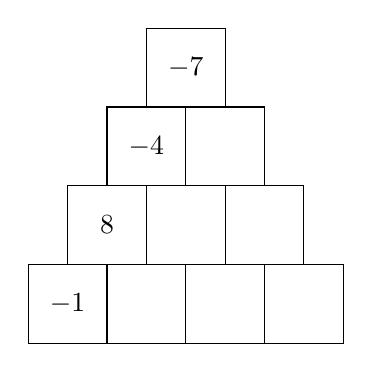
\begin{tikzpicture}
      \pyramidedenombres{4}
      \pyramideplacernombre{1}{1}{-1}
      \pyramideplacernombre{2}{1}{8}
      \pyramideplacernombre{3}{1}{-4}
      \pyramideplacernombre{4}{1}{-7}
   \end{tikzpicture}
   \;
   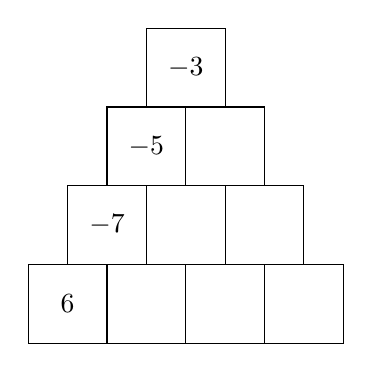
\begin{tikzpicture}
      \pyramidedenombres{4}
      \pyramideplacernombre{1}{1}{6}
      \pyramideplacernombre{2}{1}{-7}
      \pyramideplacernombre{3}{1}{-5}
      \pyramideplacernombre{4}{1}{-3}
   \end{tikzpicture}
   \ \\
   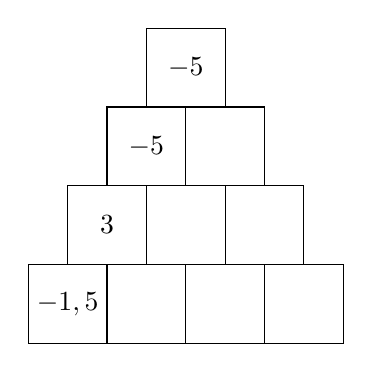
\begin{tikzpicture}
      \pyramidedenombres{4}
      \pyramideplacernombre{1}{1}{-1,5}
      \pyramideplacernombre{2}{1}{3}
      \pyramideplacernombre{3}{1}{-5}
      \pyramideplacernombre{4}{1}{-5}
   \end{tikzpicture}
   \;
   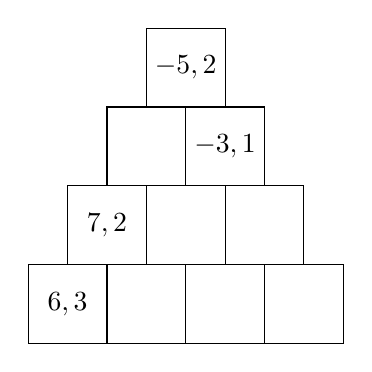
\begin{tikzpicture}
      \pyramidedenombres{4}
      \pyramideplacernombre{1}{1}{6,3}
      \pyramideplacernombre{4}{1}{-5,2}
      \pyramideplacernombre{2}{1}{7,2}
      \pyramideplacernombre{3}{2}{-3,1}
   \end{tikzpicture}
\end{exercice}

\begin{corrige}
   \ \\ [-3mm]
   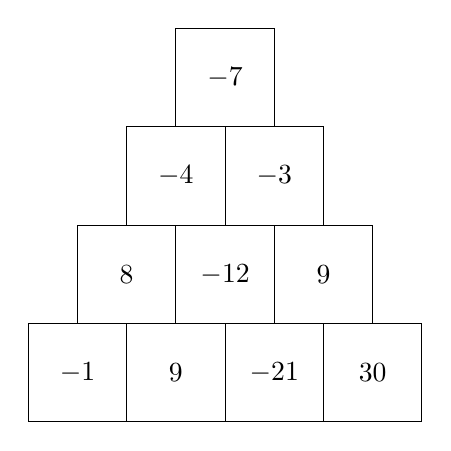
\begin{tikzpicture}[scale=1.25]
      \pyramidedenombres{4}
      \pyramideplacernombre{1}{1}{-1}
      \pyramideplacernombre{1}{2}{{\blue 9}}
      \pyramideplacernombre{1}{3}{{\blue -21}}
      \pyramideplacernombre{1}{4}{{\blue 30}}
      \pyramideplacernombre{2}{1}{8}
      \pyramideplacernombre{2}{2}{{\blue -12}}
      \pyramideplacernombre{2}{3}{{\blue 9}}
      \pyramideplacernombre{3}{1}{-4}
      \pyramideplacernombre{3}{2}{{\blue -3}}
      \pyramideplacernombre{4}{1}{-7}
   \end{tikzpicture}

   \bigskip

   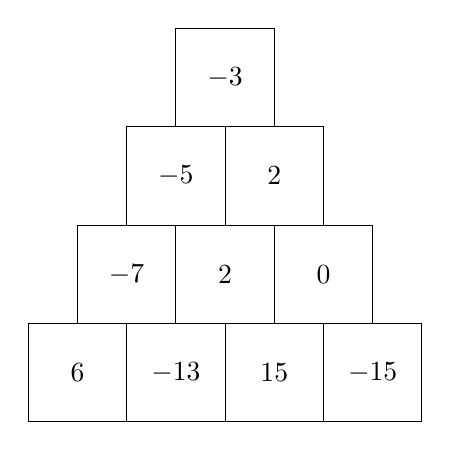
\begin{tikzpicture}[scale=1.25]
      \pyramidedenombres{4}
      \pyramideplacernombre{1}{1}{6}
      \pyramideplacernombre{1}{2}{{\blue -13}}
      \pyramideplacernombre{1}{3}{{\blue 15}}
      \pyramideplacernombre{1}{4}{{\blue -15}}
      \pyramideplacernombre{2}{1}{-7}
      \pyramideplacernombre{2}{2}{{\blue 2}}
      \pyramideplacernombre{2}{3}{{\blue 0}}
      \pyramideplacernombre{3}{1}{-5}
      \pyramideplacernombre{3}{2}{{\blue 2}}
      \pyramideplacernombre{4}{1}{-3}
   \end{tikzpicture}
   
   \bigskip
      
   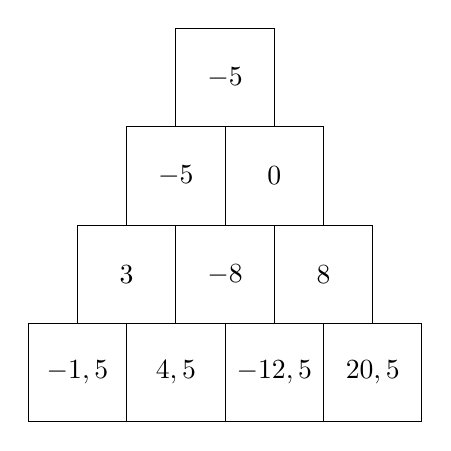
\begin{tikzpicture}[scale=1.25]
      \pyramidedenombres{4}
      \pyramideplacernombre{1}{1}{-1,5}
      \pyramideplacernombre{1}{2}{{\blue 4,5}}
      \pyramideplacernombre{1}{3}{{\blue -12,5}}
      \pyramideplacernombre{1}{4}{{\blue 20,5}}
      \pyramideplacernombre{2}{1}{3}
      \pyramideplacernombre{2}{2}{{\blue -8}}
      \pyramideplacernombre{2}{3}{{\blue 8}}
      \pyramideplacernombre{3}{1}{-5}
      \pyramideplacernombre{3}{2}{{\blue 0}}
      \pyramideplacernombre{4}{1}{-5}
   \end{tikzpicture}

   \bigskip
      
   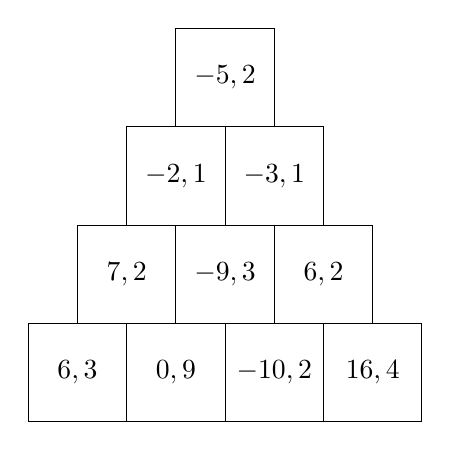
\begin{tikzpicture}[scale=1.25]
      \pyramidedenombres{4}
      \pyramideplacernombre{1}{1}{6,3}
      \pyramideplacernombre{1}{2}{{\blue 0,9}}
      \pyramideplacernombre{1}{3}{{\blue -10,2}}
      \pyramideplacernombre{1}{4}{{\blue 16,4}}
      \pyramideplacernombre{2}{1}{7,2}
      \pyramideplacernombre{2}{2}{{\blue -9,3}}
      \pyramideplacernombre{2}{3}{{\blue 6,2}}
      \pyramideplacernombre{3}{1}{{\blue -2,1}}
      \pyramideplacernombre{3}{2}{-3,1}
      \pyramideplacernombre{4}{1}{-5,2}
   \end{tikzpicture}
   
\Coupe

\corec{Décryptage}
\bigskip

   {\hautab{2}
   Premier code. \\ [2mm]
   \begin{tabular}{|p{1.8cm}|p{1.8cm}|}
      \hline
      \Large\ding{101} = \textcolor{blue}{5} & \Large\ding{40} = \textcolor{blue}{6} \\
      \hline
      \Large\ding{168} = \textcolor{blue}{3} & \Large\ding{52} = \textcolor{blue}{9} \\
      \hline
   \end{tabular}  
   \ \\ [5mm]
   Deuxième code. \\ [2mm]
   \begin{tabular}{|p{1.8cm}|p{1.8cm}|}
      \hline
      \Large\ding{101} = \textcolor{blue}{$-1$} & \Large\ding{40} = \textcolor{blue}{2} \\
      \hline
      \Large\ding{168} = \textcolor{blue}{$-4$} & \Large\ding{52} = \textcolor{blue}{5}\\
      \hline
   \end{tabular}
   \ \\ [5mm]
   Troisième code. \\ [2mm]
   \begin{tabular}{|p{1.8cm}|p{1.8cm}|p{1.8cm}|}
      \hline
      \Large\ding{101} = \textcolor{blue}{$-1$} & \Large\ding{40} = \textcolor{blue}{2} & \Large\ding{168} = \textcolor{blue}{3} \\
      \hline
      \Large\ding{36} = \textcolor{blue}{$-7$} & \Large\ding{52} = \textcolor{blue}{$-5$} \\
      \cline{1-2}
   \end{tabular}
   \ \\ [5mm]
   Quatrième code. \\ [2mm]
   \begin{tabular}{|p{1.8cm}|p{1.85cm}|p{1.8cm}|}
      \hline
      \Large\ding{101} = \textcolor{blue}{81} & \Large\ding{40} = \textcolor{blue}{$-59$} & \Large\ding{168} = \textcolor{blue}{$-25$} \\
      \hline
      \Large\ding{36} = \textcolor{blue}{47} & \Large\ding{52} = \textcolor{blue}{$-54$} \\
      \cline{1-2}
   \end{tabular}}
\end{corrige}

\end{colonne*exercice}


%%%%%%%%%%%%%%%%%%%%%%%%%%%%%%%%%%%%%%%%
%%%%%%%%%%%%%%%%%%%%%%%%%%%%%%%%%%%%%%%%
\Recreation

\enigme[Décryptage]
   Décrypter les codes suivants utilisé par l'agent Zérozérossette sachant que chaque symbole correspond à un nombre entier relatif et que la somme de chaque ligne et de chaque colonne est indiquée en bout de celle-ci. \\
   \medskip
   \begin{center}
      {\hautab{1.5}
      \begin{tabular}{*{7}{C{0.3}}}
         \Large\ding{101} & $+$ & \Large\ding{101} & $+$ & \Large\ding{40} & $=$ & \encercle{16} \\
         $+$ & & $+$ & & $+$ & & \\
         \Large\ding{168} & + & \Large\ding{168} & + & \Large\ding{168} & $=$ & \encercle{9} \\
         $+$ & & $+$ & & $+$ & & \\
         \Large\ding{40} & + & \Large\ding{52} & + & \Large\ding{168} & $=$ & \encercle{18} \\
         $=$ & & $=$ & & $=$ & & \\
         \encercle{14} & & \encercle{17} & & \encercle{12} & & \\
      \end{tabular}
      \hspace*{4cm}
      \begin{tabular}{*{7}{C{0.3}}}
         \Large\ding{101} & $+$ & \Large\ding{101} & $+$ & \Large\ding{101} & $=$ & \encercle{$-3$} \\
         $+$ & & $+$ & & $+$ & & \\
         \Large\ding{40} & + & \Large\ding{168} & + & \Large\ding{101} & $=$ & \encercle{$-3$} \\
         $+$ & & $+$ & & $+$ & & \\
         \Large\ding{52} & + & \Large\ding{52} & + & \Large\ding{168} & $=$ & \encercle{6} \\
         $=$ & & $=$ & & $=$ & & \\
         \encercle{6} & & \encercle{0} & & \encercle{$-6$} & & \\
      \end{tabular}

      \ \\ [10mm]
      
      \begin{tabular}{|p{1.8cm}|p{1.8cm}|}
         \hline
         \Large\ding{101} = & \Large\ding{40} = \\
         \hline
         \Large\ding{168} = & \Large\ding{52} = \\
         \hline
      \end{tabular}
      \hspace*{5cm}
      \vspace*{1cm}
      \begin{tabular}{|p{1.8cm}|p{1.8cm}|}
         \hline
         \Large\ding{101} = & \Large\ding{40} = \\
         \hline
         \Large\ding{168} = & \Large\ding{52} = \\
         \hline
      \end{tabular}

      \ \\ [5mm]
      
      \begin{tabular}{*{9}{C{0.3}}}
         \Large\ding{101} & $+$ & \Large\ding{40} & $+$ & \Large\ding{40} & $+$ & \Large\ding{101} & $=$ & \encercle{2} \\
         $+$ & & $+$ & & $+$ & & $+$ & \\
         \Large\ding{40} & $+$ & \Large\ding{40} & $+$ & \Large\ding{40} & $+$ & \Large\ding{168} & $=$ & \encercle{9} \\
         $+$ & & $+$ & & $+$ & & $+$ & \\
         \Large\ding{40} & + & \Large\ding{168} & + & \Large\ding{52} & $+$ & \Large\ding{36} & $=$ & \encercle{$-7$} \\
         $=$ & & $=$ & & $=$ & & $=$ & \\
         \encercle{3} & & \encercle{7} & & \encercle{$-1$} & & \encercle{$-5$} & & \\ 
      \end{tabular}
      \hspace*{2cm}
      \begin{tabular}{*{9}{C{0.3}}}
         \Large\ding{52} & $+$ & \Large\ding{52} & $+$ & \Large\ding{168} & $+$ & \Large\ding{168} & $=$ & \encercle{\!\!$-158$} \\
         $+$ & & $+$ & & $+$ & & $+$ & \\
         \Large\ding{40} & $+$ & \Large\ding{52} & $+$ & \Large\ding{36} & $+$ & \Large\ding{36} & $=$ & \encercle{\!$-19$} \\
         $+$ & & $+$ & & $+$ & & $+$ & \\
         \Large\ding{101} & + & \Large\ding{52} & + & \Large\ding{40} & $+$ & \Large\ding{52} & $=$ & \encercle{\!$-86$} \\
         $=$ & & $=$ & & $=$ & & $=$ & \\
         \encercle{\!$-32$} & & \encercle{\!\!$-162$} & & \encercle{\!$-37$} & & \encercle{\!$-32$} & & \\ 
      \end{tabular}

     \ \\ [10mm]
     
      \begin{tabular}{|p{1.8cm}|p{1.8cm}|p{1.8cm}|}
         \hline
         \Large\ding{101} = & \Large\ding{40} = & \Large\ding{168} = \\
         \hline
         \Large\ding{36} = & \Large\ding{52} = \\
         \cline{1-2}
      \end{tabular}
      \hspace*{2cm}
      \begin{tabular}{|p{1.8cm}|p{1.8cm}|p{1.8cm}|}
         \hline
         \Large\ding{101} = & \Large\ding{40} = & \Large\ding{168} = \\
         \hline
         \Large\ding{36} = & \Large\ding{52} = \\
         \cline{1-2}
      \end{tabular}}
   \end{center}

